\section{Introduction}
\label{sec:intro}

This work contains a collection of applications of the 
Discrete Gauss-Bonnet theorem.
I hope that the number of applications continues to grow,
please share any that you feel
ought to  be included\footnote{\text{bradleymccoy@montana.edu}}.
Here we emphasize applications of the \emph{discrete} Gauss-Bonnet
theorem. Several applications of the continuous version of the theorem
are given in \cite{doc76}.
For applications of the Gauss-Bonnet theorem in physics see \cite{tirado-physics-apps}.


To get a sense of the types of problems we will encounter,
let's consider a simple special case of the Gauss-Bonnet theorem.
\begin{theorem}\label{thm:triangle}
In the plane, the sum of the interior angles of a triangle is $\pi$.
\end{theorem}
\begin{proof}
Draw a line parallel to one edge through the opposite vertex.
By alternating interior angles in the plane, the sum of the angles
in the triangle equal  a straight line.
See \figref{angles} for an illustration. 



\begin{figure}[htb]
\centering
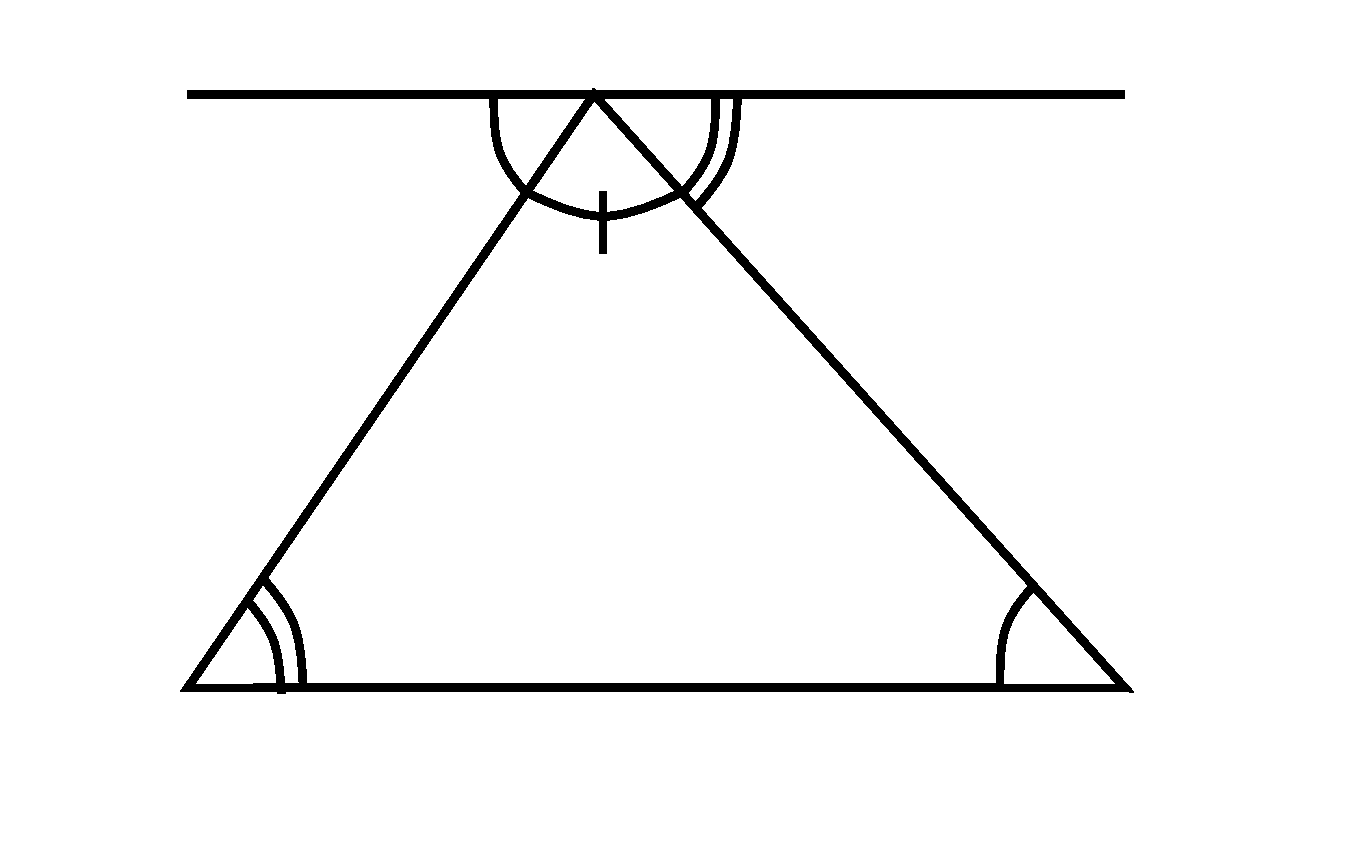
\includegraphics[width=.3\textwidth]{sec-1-and-2/interior-angles-triangle}
\caption{A proof that, in the plane, the sum of the angles of a triangle is $\pi$.}
\label{fig:angles}
\end{figure}

\end{proof}

Note the sum of the angles of a triangle does not
depend on certain properties of the  triangle, such as the orientation in the plane or
the scale factor of the triangle.


Even this simple version of the theorem is useful.
Consider any simple polygon $P$ on $n$ vertices. 
What is the sum of the interior angles of $P$?
One could measure each angle, but if $n$ is large they would eventually
get tired.
Instead, we notice that any polygon with $n$ vertices can be
triangulated with $n-2$ triangles. This can be proved by induction.
Thus, when we traverse $P$ we go around $n-2$ triangles each contributing
$\pi$.
As a corollary to \thmref{triangle} we have
\begin{corollary}\label{cor:angles}
In the plane, any simple polygon $P$ with $n$ vertices,
the sum of the interior angles of $P$ is $(n-2)\pi$.

\end{corollary}

Now, we do not need to measure any angles to find
the sum of  the interior angles of a polygon. We can simply
count the vertices. What savings!

This paper is organized as follows:
in \secref{cast} we introduce definitions and notation that will be used
throughout the paper and state the theorem,
in \secref{proof}, we present a proof of the theorem, and in each of the remaining $n$
sections we present an application of the theorem.
In general, the sections containing applications are ordered from simpler to more technical,
and are independent.


